% source: https://www.cs.cmu.edu/~dst/WordEmbeddingDemo/tutorial.html
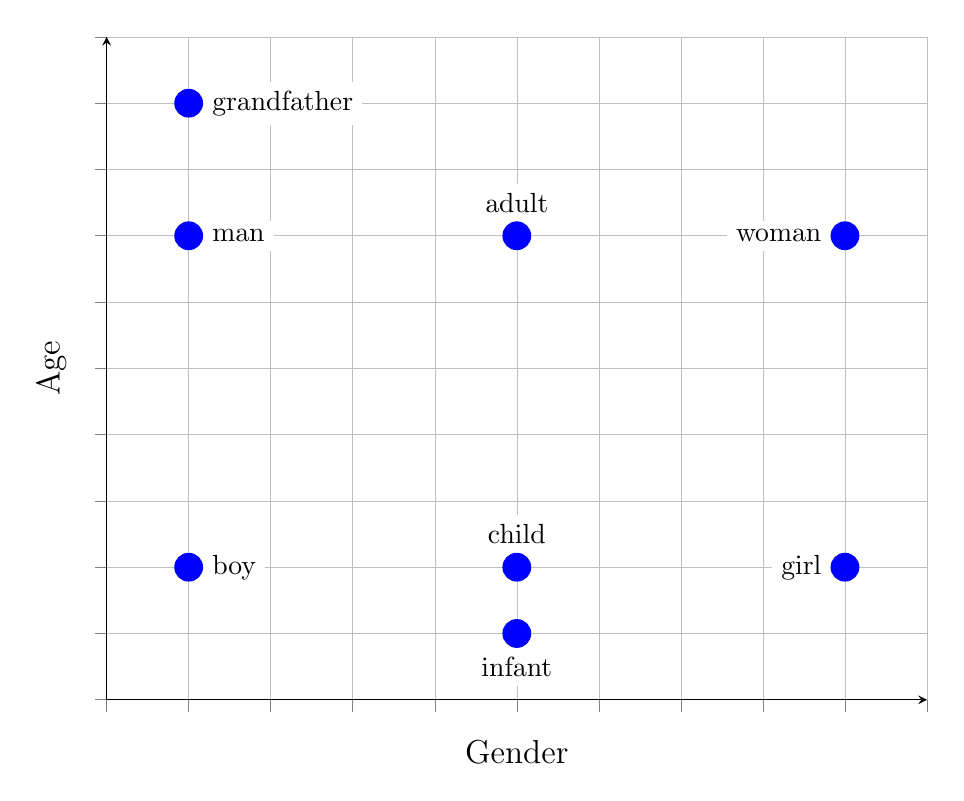
\begin{tikzpicture}
  \begin{axis}[
      width=12cm, height=10cm,
      xlabel={Gender}, ylabel={Age},
      xmin=0, xmax=10, ymin=0, ymax=10,
      xtick={0,1,...,10}, ytick={0,1,...,10},
      xticklabel={\empty}, yticklabel={\empty},
      grid=both,
      grid style={line width=.1pt, draw=gray!30},
      major grid style={line width=.2pt,draw=gray!50},
      axis lines=left,
      tick align=outside,
      enlargelimits=false,
      label style={font=\large},
      title style={font=\LARGE, yshift=1em},
      every tick label/.append style={font=\small},
    ]

    % Plot the points
    \addplot[
      only marks,
      mark=*,
      mark size=5pt,
      blue,
    ] coordinates {
        (1,9)   % grandfather
        (1,7)   % man
        (1,2)   % boy
        (5,7)   % adult
        (5,2)   % child
        (5,1)   % infant
        (9,7)   % woman
        (9,2)   % girl
      };

    % Add labels
    \node[fill=white, anchor=west, xshift=5pt, font=\normalsize] at (axis cs:1,9)  {grandfather};
    \node[fill=white, anchor=west, xshift=5pt, font=\normalsize] at (axis cs:1,7)  {man};
    \node[fill=white, anchor=west, xshift=5pt, font=\normalsize] at (axis cs:1,2)  {boy};
    \node[fill=white, anchor=south, yshift=5pt, font=\normalsize] at (axis cs:5,7)  {adult};
    \node[fill=white, anchor=south, yshift=5pt, font=\normalsize] at (axis cs:5,2)  {child};
    \node[fill=white, anchor=north, yshift=-5pt, font=\normalsize] at (axis cs:5,1)  {infant};
    \node[fill=white, anchor=east, xshift=-5pt, font=\normalsize] at (axis cs:9,7)  {woman};
    \node[fill=white, anchor=east, xshift=-5pt, font=\normalsize] at (axis cs:9,2)  {girl};
  \end{axis}
\end{tikzpicture}